\documentclass[a4paper]{report}

\usepackage{fontspec}				% utf-8 support
\usepackage{graphicx}				% To include images
\usepackage[margin=2.5cm]{geometry}	% Better margins
\usepackage[catalan]{babel}			% Catalan sections support
\usepackage[hidelinks]{hyperref}	% Autoref support
\usepackage{setspace}				% Allows to set a specific stretch
\usepackage{float}
\usepackage{gensymb}
\usepackage{multirow}
\usepackage{longtable}
\usepackage{tikz}
\usepackage{pgfplots}

\addto\captionscatalan{\renewcommand{\chaptername}{Pràctica}}

\setlength{\parindent}{0pt}
\setlength{\parskip}{0.2cm}

\title{\textsc{\huge Tecnologia de Selecció de Materials} \\
        Informe pràctiques}
\author{Marta Gomis Domènech \and 
    Joan Marcè Igual \and 
    Èlia Mateu Barriendos \and 
    Esteve Tarragó Sanchís \and 
    Néstor Tuneu Arroyo}

\begin{document}

\begin{titlepage}
    \centering
    \vspace{1cm}
    
\includegraphics[width=0.25\textwidth]{images/etseib}
    \par\vspace{1cm}
    \textsc{ \LARGE Escola Tècnica Superior d'Enginyeria \\[1em] 
        Industrial de Barcelona}
    \par\vspace{2cm}
    \textbf{\Huge Tecnologia i Selecció de Materials}
    \par\vspace{2cm}
    {\LARGE Informe pràctiques}
    \vfill
    \begin{flushright}
        \large
        Marta Gomis Domènech \par
        Joan Marcè Igual \par
        Èlia Mateu Barriendos \par
        Esteve Tarragó Sanchís \par
        Néstor Tuneu Arroyo
    \end{flushright}
\end{titlepage}

\tableofcontents

\chapter{Assaig a tracció}

\section{Proveta metà\l. lica }

La \autoref{fig:traccio-metalica-grafic-proveta} correspon al resultat de l'assaig a tracció de la proveta metà\l.lica de 6 mm de diàmetre inicial, marcada amb separacions de 10 mm per estimar posteriorment paràmetres de ruptura. 

\begin{figure}[hb]
    \centering
    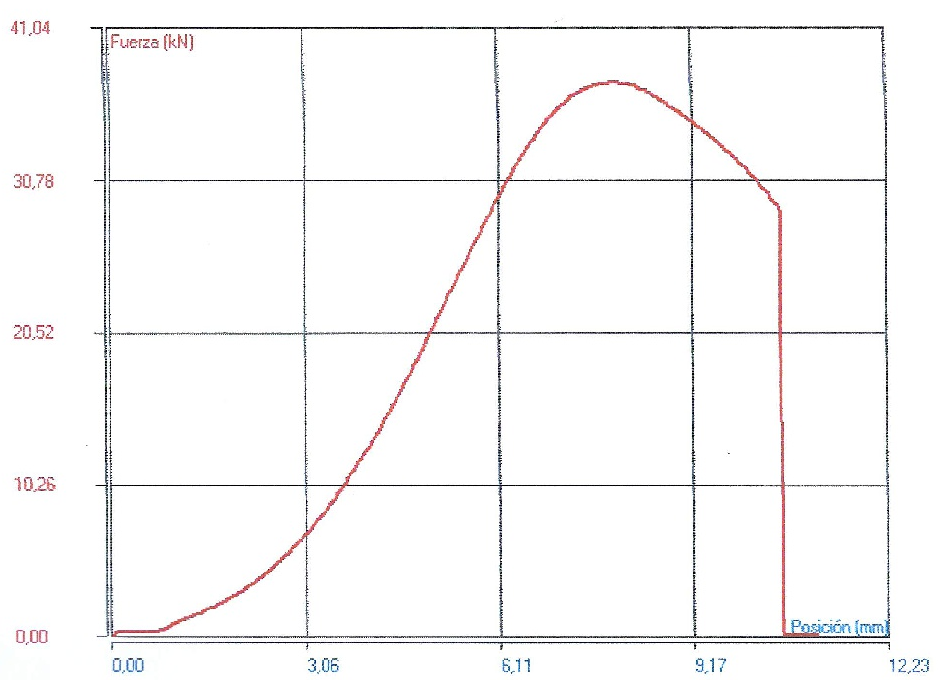
\includegraphics[width=0.9\textwidth]{images/traccio/metalica-grafic-proveta}
    \caption{Gràfic F-d de la proveta metà\l.lica}
    \label{fig:traccio-metalica-grafic-proveta}
\end{figure}

Abans de concretar algunes qüestions sobre l'assaig, a priori ja es poden extreure algunes conclusions del únicament utilitzant el gràfic:
\begin{itemize}
    \item  S'ha produït la ruptura del material. Això ho poden notar amb la línia vertical final en el gràfic.
    \item  La peça ha relliscat al principi, com queda indicat a la línia horitzontal inicial del gràfic. Aquest fenomen retarda l'aparició de la zona elàstica del material, caracteritzada per una zona de pendent constant, que es troba aproximadament entre els 4 mm i els 6,11 mm de desplaçament dels capçals de la màquina.
    \item  El material ha patit estricció. La zona de pendent negatiu indica que la secció del material està disminuint, doncs es necessita menys força per continuar deformant.
    \item  La ruptura és dúctil. Es pot corroborar analitzant la superfície de ruptura.
\end{itemize}

\subsection{El fenomen de l'estricció}

Durant l'assaig a tracció, en superar el valor màxim de força, el material plastifica i comença a deformar apareixent un coll. Aquesta deformació axial genera una contracció radial que redueix la secció de la proveta. La màquina d'assaigs a tracció, aplica força per moure's a velocitat constant, per tant, com la secció disminueix aplica menys força per continuar deformant a la mateixa velocitat, fins arribar a la fallida per ruptura de la peça.

A la \autoref{fig:traccio-metalica-grafic-proveta} això es tradueix en una regió de pendent negativa entre el valor màxim de força i el moment de la fallida, tal com s'ha comentat al principi.

Com el material és crista\l.lí, el material no deforma gaire abans de trencar.

\subsection{Morfologia de la fractura}
Per estudiar la morfologia de la ruptura és essencial la fixar-se en la superfície de fractura. El primer que s'observa en una de les parts és un contorn ondulat que indica que el material ha deformat abans de trencar i per tant la ruptura és dúctil. Aquest contorn ondulat té major diàmetre que el diàmetre d'estricció màxima, per tant, es pot concloure que aquest fragment ha fallat per forces tangencials, abans de trencar definitivament.

Un altre indicador de ruptura dúctil és la rugositat de les superfícies, que s'observa a ull nu malgrat la contaminació d'aquestes. De tota manera, les peces encaixen amb relativa facilitat, per tant el material no deforma de manera considerable com els polímers, dels quals es parlarà més endavant.

Aquestes consideracions es veuen i\l.lustrades a la \autoref{fig:traccio-metalica-superficie-ruptura}, que és una fotografia de les dues superfícies de ruptura. 

\begin{figure}[ht]
    \centering
    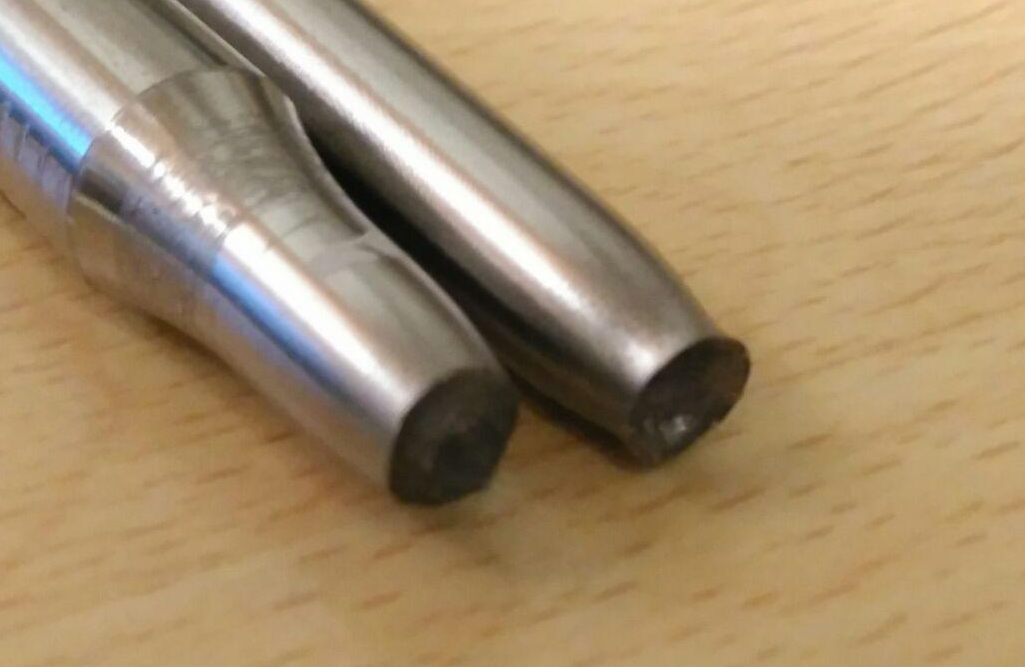
\includegraphics[width=0.5\textwidth]{images/traccio/metalica-superficie-ruptura}
    \caption{Superfícies de ruptura de la proveta metà\l.lica}
    \label{fig:traccio-metalica-superficie-ruptura}
\end{figure}

\subsection{Paràmetres de ruptura}

Utilitzant les marques inicials de la proveta, les dimensions finals i el gràfic F-d, es poden obtenir els següents paràmetres: límit elàstic, càrrega màxima, allargament a la ruptura (\%) i estricció (\%).

La càrrega màxima és una mesura directa del gràfic, sent el màxim valor d'aquesta. Mitjançant mètodes d'aproximació gràfica, s'ha estimat que aquest valor és $38,43 \ kN$.

El límit elàstic real es defineix com el punt on el material comença a plastificar. El límit elàstic convencional tolera un $0,2\%$ de deformació. Aquests dos valors són representatius del valor del límit elàstic i es poden estimar sempre que es puguin mesurar les deformacions. 

Donat que no es disposava d'extensòmetre es farà l'aproximació del valor del límit elàstic com el quocient entre el valor de força abans d'abandonar el règim elàstic entre l'àrea inicial. Aprofitant que les deformacions en la proveta metà\l.lica són reduïdes, s'ha considerat que és una estimació suficientment correcte.

S'ha pres el valor de força (estimat també gràficament) de $28,50 \ kN$, el que suposa una tensió de límit elàstic de $1007,98 \ N/mm^2$. S'ha suposat que la secció de la proveta és perfectament circular.

Quant a l'allargament a la ruptura, la distància entre les marques entre les quals s'ha produït la ruptura ha passat de $10 \ mm$ a $13,6 \ mm$, per tant, l'allargament és d'un $36\%$.

Per últim, el diàmetre final de la proveta, mesurada amb una precisió de $0,1 \ mm$ és de $5 \ mm$, per tant, l'estricció és d'un $30,56\%$.

\chapter{Tractaments tèrmics}

L'objectiu d'aquesta pràctica és determinar l'efecte de tres tractaments tèrmics en les propietats d'un acer F-1140 (0,45\% C, 0,65\% Mn, 0,25\% Si, ≤0,03\% P, ≤0,03\% S). 

Es disposa de tres provetes d'aquest acer i cada una d'elles es sotmet a un tractament tèrmic: tremp, tremp i revingut a 600ºC o normalitzat. Posteriorment, se'n mesura la duresa (resistència del material a ser deformat plàsticament) mitjançant el duròmetre Hoytom (es prenen tres valors i es fa la mitjana) i la resiliència (energia de deformació elàstica que pot ser emmagatzemada per un cos) amb el pèndul Charpy. Els valors obtinguts per a cada proveta es recullen a la \autoref{tab:tract-assaigs}:


\begin{table}[H]
	\centering
	\begin{tabular}{|r|lrr|}
		\hline
		Proveta & Tractament tèrmic & Duresa  & Resiliència \\
		\hline
		1 & Tremp & 46,7 HRC & 0 $kg \cdot m$ \\
		2 & Tremp i revingut a 600ºC & 79,3 HRB & 7,2 $kg \cdot m$ \\
		3 & Normalitzat & 59,7 HRB & 3,8 $kg \cdot m$ \\
		\hline
	\end{tabular}
	\caption{Resultats dels assaig de duresa i resiliència}
	\label{tab:tract-assaigs}
\end{table}

\section{Tremp}
La primera proveta es sotmet a un tremp en aigua des de la temperatura de 860ºC. Aquest tractament tèrmic és un mecanisme d'enduriment i implica un refredament molt ràpid i, per tant, fora de l'equilibri. L'estructura generada és la martensita: es tracta d'una solució sòlida sobresaturada en C en una xarxa tetragonal centrada en el cos (BCT). Així doncs, aquesta estructura distorsionada es genera fruït de la transformació adifusional de l'austenita i es caracteritza per una elevada duresa (50-70 HRC), resistència i fragilitat donat que reté moltes tensions internes. 

\section{Tremp i revingut a 600ºC (Bonificat)}

Tot i que el tremp proporciona una elevada duresa, el principal inconvenient és la també elevada fragilitat que l'acompanya, ja que la martensita és una estructura molt tensionada. Per tal que una peça trempada pugui tenir posteriors aplicacions, cal aplicar-li un tractament de revingut que elimini aquestes tensions. L'objectiu del revingut és, per tant, augmentar la tenacitat i disminuir la fragilitat, tot i que això implica que minvin la duresa i la resistència. L'operació, que com s'ha dit es realitza immediatament després d'un tremp, consisteix en escalfar el' material durant un temps determinat a una temperatura inferior a la d'austenització. 

Hi ha dos possibles revinguts, el baix i l'alt, en funció de la temperatura a la que es dugui a terme el tractament. El revingut baix (180-220ºC) només s'aplica en tremps per enduriment superficial, ja que manté una elevada duresa però baixa tenacitat. El revingut alt (450-650ºC), que és el que s'ha aplicat a la pràctica, augmenta la tenacitat en detriment de la duresa i la resistència. La microestructura final està composta per grans de cementita (duresa $\approx$ 700HB) en una matriu ferrítica (duresa $\approx$ 80HB).

\section{Normalitzat}
El normalitzat és un tractament tèrmic que té per objectiu eliminar les tensions internes i homogeneïtzar l’estructura de les peces a les quals s’aplica. Consisteix en l’escalfament a una temperatura per sobre la d’austenització (en el cas de la pràctica, 860ºC) amb un temps de manteniment relativament llarg (30min-1h per polzada de gruix),  per tal que tota la peça assoleixi la mateixa temperatura i no es generin diferències microestructurals; i finalment un refredament lent (a l’aire). És un tractament que sol ser previ al tremp, amb l’objectiu de que el material recuperi les seves condicions ``normals" que es poden haver vist modificades degut a processos previs de mecanitzat; per exemple, el treball en fred. Aquest procés genera acritud en el material, augmenta la duresa i la fragilitat, de manera que si es pretén aplicar un tremp és convenient disminuir prèviament les tensions internes generades i homogeneïtzar la microestructura. 

\section{Discussió dels resultats}
Les provetes es poden ordenar de la següent manera veient els resultats en duresa i resiliència obtinguts en els assaigs:

\begin{table}[H]
	\centering
	\begin{tabular}{lr}
		\textbf{Duresa} & Tremp > Revingut > Normalitzat \\
		\textbf{Resiliència} & Revingut > Normalitzat > Tremp
	\end{tabular}
\end{table}

Pel que fa a la duresa, s’observa que els resultats són coherents en relació a les microestructures generades per cada tractament. La proveta trempada presenta el valor més elevat de duresa ja que, com s’ha dit, la martensita és una estructura molt tensionada i això li aporta una elevada duresa i fragilitat. Cal comentar que la duresa de la martensita està entre 50 i 70 HRC i que el resultat obtingut és lleugerament inferior a aquest rang. Això es pot deure a que el temps entre treure la proveta del forn i submergir-la en aigua va ser més llarg del que seria idoni. En quant a les provetes sotmeses a revingut i normalitzat, en no contenir martensita, presenten valors inferiors de duresa. Pel que fa a la proveta revinguda, en tant que prové d’una estructura martensítica, té una duresa superior a la normalitzada.

Pel que fa a la resiliència, s’observa que el tremp en presenta un valor nul ja que es tracta d’una estructura mol fràgil i tensionada i, per tant, no pot emmagatzemar pràcticament energia de deformació elàstica. Tot i que la proveta revinguda prové d’una estructura martensítica i això pot dur a pensar que hauria de ser menys resilient que la normalitzada, cal tenir en compte que al tornar a ser escalfada fins a 600ºC, alhora que els valors de la duresa i resistència disminueixen, la tenacitat augmenta notablement (la tenacitat està molt correlacionada amb la resiliència, ja que es tracta de l’energia que és capaç d’emmagatzemar el material abans de trencar). És per aquest motiu que el normalitzat, que només consisteix en un refredament lent, presenta un valor de resiliència inferior al revingut.

Les superfícies de ruptura de les tres provetes (\autoref{fig:tract-ruptures}) confirmen aquestes conclusions.

\begin{figure}[H]
	\centering
	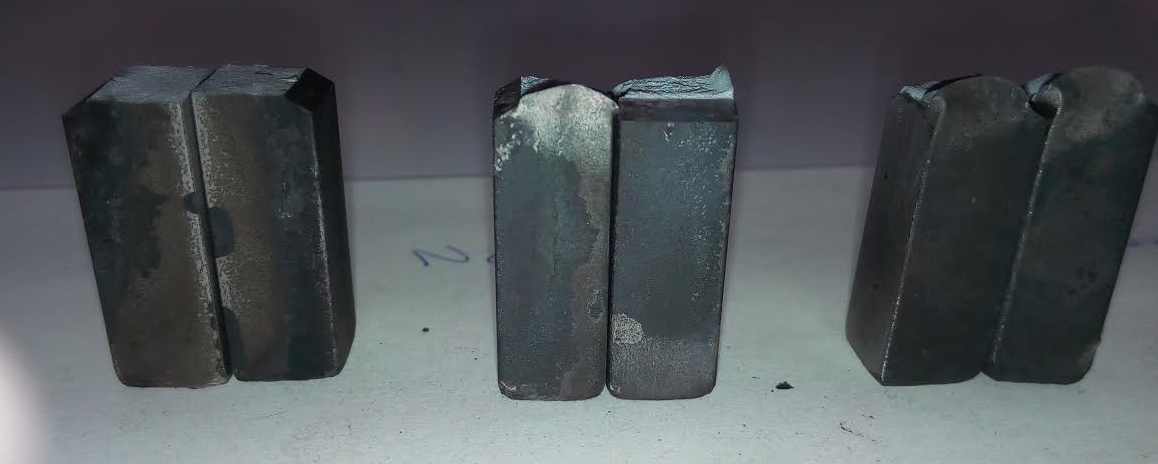
\includegraphics[width=0.8\textwidth]{images/tractaments/ruptures}
	\caption{Superfícies de ruptura de les provetes. D'esquerra a dreta: tremp, normalitzat i revingut}
	\label{fig:tract-ruptures}
\end{figure}

S’observa que la superfície de ruptura de la proveta trempada és llisa i neta, característica dels materials fràgils. Pel que fa a la revinguda, presenta uns llavis majors que la normalitzada, ja que aquesta és menys tenaç (la tenacitat sol ser un indicador de ductilitat).

\chapter{Trempabilitat (assaig Jominy)}
L’objectiu d’aquesta pràctica és determinar la corba de trempabilitat d’un acer F-1140, de la mateixa composició que l’acer utilitzat en la Pràctica 2: 0.45\% C, 0.65\% Mn, 0.25\% Si, 0.03\% P i 0.03\% S. Aquesta proporció dels elements aliants de l’acer afectarà significativament a la seva trempabilitat.

La trempabilitat d’un acer indica la seva predisposició a deixar-se penetrar pel tremp, i es mesura mitjançant el gradient de dureses que hi ha des de la superfície d’una peça fins al seu nucli. En aquesta pràctica es realitza l’assaig Jominy, que és el mètode més utilitzat per definir i mesurar la trempabilitat dels acers. L’assaig consisteix en escalfar una proveta cilíndrica de $25 mm$ de diàmetre i $100 mm$ de longitud fins a la temperatura d’austenització: $860 \degree C$. Tot seguit es realitza el tremp a la cara inferior de la proveta refredant-la amb un raig d’aigua vertical. La cara trempada de la proveta representa la superfície de la peça i la cara oposada en representa el nucli. 

\section{Evolució de la duresa en funció de la distància a la base trempada}
Es mesuren les dureses en diferents punts al llarg de la generatriu del cilindre mitjançant el duròmetre Hoytom per tal d’obtenir la corba de trempabilitat de l’acer. Per a cada distància de la base trempada es realitzen dues mesures i se'n fa la mitjana. Les mesures més properes a la cara trempada es realitzen amb la punta de con diamant (HRC) per tal de no malmetre la punta de bola en cas que l’acer sigui més dur que aquesta. Posteriorment, quan la duresa ja ha disminuït una mica, es canvia la punta de diamant per la de bola $1/16"$ (HRB). Els valors tabulats indiquen que amb la punta de diamant el duròmetre Hoytom s’ha d’ajustar a una càrrega de 150 kp (aproximadament $1471 N$) i en el cas de la bola $1/16"$ la càrrega s’ha d’ajustar a $100 kp$ (aproximadament $981 N$). S’obtenen els valors següents de dureses Rockwell, els quals es converteixen mitjançant els valors tabulats a duresa Vickers per tal de poder-los comparar:

\begin{longtable}{|r|rrr|r|}
	\hline
	\multirow{2}{*}{\textbf{Distancia (mm)}} & \multicolumn{3}{c|}{Duresa Rockwell (HR)} & \multirow{2}{*}{Duresa Vickers (HV)} \\
	\cline{2-4}
	& Mesura 1 & Mesura 2 & Mitjana &  \\
	\hline
	\textbf{1,5} & 47 & 43 & 45 & 446 \\
	\textbf{3} & 44 & 46 & 45 & 446 \\
	\textbf{5} & 48 & 42 & 45 & 445 \\
	\textbf{7} & 43 & 47 & 45 & 443 \\
	\textbf{9} & 45 & 44 & 44,5 & 439 \\
	\textbf{11} & 46 & 42 & 44 & 434 \\
	\textbf{13} & 41 & 46 & 43,5 & 430 \\
	\textbf{15} & 42 & 44 & 43 & 423 \\
	\textbf{20} & 38 & 43 & 40,5 & 396 \\
	\textbf{25} & 39 & 33 & 36 & 355 \\
	\textbf{30} & 28 & 29 & 28,5 & 290 \\
	\textbf{35} & 100 & 96 & 98 & 240 \\
	\textbf{40} & 89 & 90 & 89,5 & 190 \\
	\textbf{45} & 88 & 84 & 86 & 175 \\
	\textbf{50} & 86 & 84 & 85 & 170 \\
	\textbf{55} & 83 & 83 & 83 & 165 \\
	\textbf{60} & 84 & 81 & 82,5 & 163 \\
	\textbf{65} & 82 & 81 & 81,5 & 160 \\
	\textbf{70} & 81 & 84 & 82,5 & 163 \\
	\textbf{75} & 79 & 81 & 80 & 155 \\
	\textbf{80} & 80 & 81 & 80,5 & 156 \\
	\textbf{85} & 80 & 79 & 79,5 & 153 \\
	\hline
	\caption{Valors obtinguts durant l'assaig de duresa}
\end{longtable}

La primera columna correspon a la distància fins la cara trempada de la proveta. Com es pot observar, els 11 primers valors s’han mesurat en l’escala HRC i la resta en l’escala HRB. S’ha acabat l’assaig en el moment que s’ha observat clarament la tendència constant de la duresa de la proveta (aproximadament a partir dels 5 cm de distància fins la base trempada. Es representa tot seguit la corba de trempabilitat de l’acer F-1140:

% M'he quedat aqui!!!!!!!!!!!!!!
\begin{figure}[H]
	\centering
	\begin{tikzpicture}
		\begin{axis}[
				grid = both,
				grid style = { line width = .1pt, draw = gray!10 },
				major grid style = {line width = .2pt, draw = gray!50 },
				width = 0.8\textwidth, height = 0.7\textwidth,
				xtick = {}, ytick = {},
				xlabel = Distància (mm),
				ylabel = Duresa VR,
				minor y tick num = 4,
				minor x tick num = 3,
				axis on top
			]
			\addplot+[smooth] table[x=D,y=H] {data/jominy/duresa.csv};
		\end{axis}
	\end{tikzpicture}
	\caption{Duresa mesurada a la peça en funció de la distància}
\end{figure}

\end{document}